%\documentclass[9pt, aspectratio=169]{beamer}
\documentclass[9pt, handout, aspectratio=169]{beamer}		% For use when we want to skip \pause commands exporting
\usetheme{PedroRiveroANLwide}

%\setbeameroption{show notes}
%\setbeameroption{show only notes}
\setbeamerfont{note page}{size=\fontsize{0.2cm}{0.1cm}}

%%%%%%%%%%%%%%%%%%%%%%%%%%%%%%%%%%%%%%%%%%%%
%%%%%%%%%%							  TITLE								%%%%%%%%%%
%%%%%%%%%%%%%%%%%%%%%%%%%%%%%%%%%%%%%%%%%%%%

\title{Quantum Computing of the Deuteron Binding Energy}
\subtitle{Improving on \href{https://arxiv.org/abs/1801.03897}{arXiv:1801.03897}}
\author{Pedro Rivero}
\newcommand{\mail}{priveroramirez@anl.gov}
\date{\emph{\small{\today}}}
\institute{Argonne National Laboratory\\ Illinois Institute of Technology\\
\href{mailto:\mail}{\nolinkurl{\mail}}}
\newcommand{\website}{www.phy.anl.gov}

\begin{document}
\justify
\setlength{\abovedisplayskip}{0pt}
\setlength{\belowdisplayskip}{12pt}
\setlength{\abovedisplayshortskip}{0pt}
\setlength{\belowdisplayshortskip}{12pt}

	\begin{frame}[plain,t]
		\titlepage
	\end{frame}

	\begin{frame}[c]{Contents Overview}
%		\begin{multicols}{2}
%  			\tableofcontents
%		\end{multicols}
		\tableofcontents
	\end{frame}

%%%%%%%%%%%%%%%%%%%%%%%%%%%%%%%%%%%%%%%%%%%%
%%%%%%%%%%							  BODY								%%%%%%%%%%
%%%%%%%%%%%%%%%%%%%%%%%%%%%%%%%%%%%%%%%%%%%%

\section{Introduction}

	\begin{frame}{What is Quantum Computing?}

		Quantum Computing is the application of \textbf{Quantum Information Science (QIS)} to the development of \textit{machines} capable of performing operations and calculations based on quantum logic instead of the usual classical logic.

		\medskip

		The usefulness of this kind of computation lays not only on the ability to engineer exponentially faster machines, but also on things such as being able to \textbf{efficiently simulate nature at the quantum level}, or creating encryption systems which are fundamentally secure.

		\medskip

		\begin{multicols}{2}

			\underline{\textbf{CLASSICAL LOGIC}}\\
			Set Theory (Boolean algebra)

			\medskip

			\begin{itemize}
				\item \textbf{AND} $\quad \Rightarrow \quad A \cup B$
				\item \textbf{OR} $\quad \Rightarrow \quad A \cap B$
				\item \textbf{NOT} $\quad \Rightarrow \quad \overline{A}$
				\item \textbf{XOR} $ \quad \Rightarrow \quad A \cap B - A \cup B$
			\end{itemize}

			\columnbreak

			\underline{\textbf{	QUANTUM LOGIC}}\\
			Quantum Theory (Non-Commutative)

			\medskip

			\begin{itemize}
				\item \textbf{Probabilistic measurement}
				\item \textbf{Measurement causes disturbance}
				\item \textbf{Superposition}
				\item \textbf{Entanglement}
				\item \textbf{Uncertainty principle}
			\end{itemize}

		\end{multicols}

	\end{frame}

%%%%%%%%%%%%%%%%%%%%%%%%%%%%%%%%%%%%%%%%%%%%

	\subsection{The Abacus Effect}

	\begin{frame}{The Abacus Effect}

		To try to understand the power of Quantum Computing in abstract, we can resort to what might be called \textbf{"The Abacus Effect"}.

		\medskip

		Before the abacus was invented, the only way of counting was through a "thermometer-like" scale, which was highly inefficient as it meant adding one physical bead per unit. The abacus did something great: it introduced the concept of \textbf{digits}, which was later put into an even more concise notation by the Arabs through the introduction of \textbf{numerals}.

		\medskip

		This means that, instead of counting up to $N$ using $N$ raw elements, we can count using only $\text{log}_b (N)$ abacus elements ---where $b$ is the base of our number system (i.e. the amount of beads per row in the abacus). Therefore, for $b\geq2$, the abacus introduced an \textbf{exponential decrease in resource requirements} to represent the exact same thing.

		\medskip

		Quantum computers do something analogous. To represent the quantum state of a system made out of $N$ subsystems ---each of which with $b$ degrees of freedom--- we would usually need $b^N$ classical elements (i.e. numbers). By using quantum systems for this representation, we would only need $N$ quantum elements (i.e. each subsystem). Again, an exponential decrease in resource requirements.

	\end{frame}

%%%%%%%%%%%%%%%%%%%%%%%%%%%%%%%%%%%%%%%%%%%%

	\subsection{Quantum Software}

	\begin{frame}{Quantum Software: IBM's Qiskit}

		Working with quantum systems is extremely difficult, and in many cases very expensive, this makes quantum computing research unavailable to many groups and institutions. In order to solve this problem, IBM has developed \textbf{Qiskit}, a python framework for quantum computation and quantum information.

		\medskip

		This framework allows the construction of quantum circuits ---today's most common way of representing quantum computation--- for running using different backends. These backends range from simulators to actual quantum devices accessible on the cloud through the IBMQ API included in Qiskit. It also includes tools for handling noise and error correction, developing quantum based applications and tools, or making use of well known, pre-programmed algorithms. It also allows work through different levels of abstraction, from microwave pulses on hardware to high level algorithm implementation.

	\end{frame}

%%%%%%%%%%%%%%%%%%%%%%%%%%%%%%%%%%%%%%%%%%%%
%%%%%%%%%%%%%%%%%%%%%%%%%%%%%%%%%%%%%%%%%%%%

\section{Case Study}

	\begin{frame}{Case Study}

		As a starting point we decided to reproduce the paper \textbf{Cloud Quantum Computing of an Atomic Nucleus} (\href{https://arxiv.org/abs/1801.03897}{arXiv:1801.03897}) by Dumitrescu \textit{et al.}

		\medskip

		In this paper, IBM's QX5 quantum computer was used to simulate the \textbf{deuteron binding energy}, through a Hamiltonian from pionless effective field theory:

		\begin{align*}
			H_N = \sum^{N-1}_{n,n'=0} \mel{n'}{(T+V)}{n}a^{\dagger}_{n'}a_{n}
		\end{align*}

		Where $N$ is the basis dimension for a discrete variable representation in the harmonic oscillator basis.

	\end{frame}

%%%%%%%%%%%%%%%%%%%%%%%%%%%%%%%%%%%%%%%%%%%%

	\subsection{Hamiltonian Mapping}

	\begin{frame}{Hamiltonian Mapping onto qubits}

		In order to simulate a quantum system on a quantum computer, we need to map its Hamiltonian onto the qubits of the device. To do so, in this case, we can use the \textbf{Jordan-Wigner transformations} which map the creation/annihilation operators onto Pauli matrices. This is necesarry as no direct measurement of a general quantum operator can be performed in a quanutm computer. However, it is possible to perform Pauli measurements with ease.

		\begin{align*}
			a^{\dagger}_{n} \rightarrow \frac{1}{2} \left[ \prod^{n-1}_{j=0} -Z_j \right] (X_n - i Y_n)
			\hspace{40pt}
			a_{n} \rightarrow \frac{1}{2} \left[ \prod^{n-1}_{j=0} -Z_j \right] (X_n + i Y_n)
		\end{align*}

		Where a spin up $\ket{\uparrow}$ on qubit $n$ represents zero deuteron in state $\ket{n}$, and a spin down $\ket{\downarrow}$ one deuteron. For different values of $N$, this returns:

		\begin{align*}
			H_1 &= 0.218291(Z_0 - I) \quad \Rightarrow \quad E_1 = \mel{\downarrow}{H_1}{\downarrow} \simeq -0.436 \text{MeV} \\
			H_2 &= 5.906709 I + 0.218291 Z_0 - 6.125 Z_1 - 2.143304(X_0 X_1 + Y_0 Y_1) \\
			H_3 &= H_2 + 9.625(I-Z_2) - 3.913119(X_1 X_2 + Y_1 Y_2) \\
			&\cdots
		\end{align*}

		\vspace{-20pt}

	\end{frame}

%%%%%%%%%%%%%%%%%%%%%%%%%%%%%%%%%%%%%%%%%%%%

	\subsection{Unitary Coupled Cluster}

	\begin{frame}{Unitary Coupled Cluster}

		To determine ground-state energy we first need to know the region of Hilbert-space representing valid states of our quantum system. Then, we can use the \textbf{Unitary Coupled Cluster ansatz}. For this, we define unitary operators entangling two and three orbitals:

		\begin{align*}
			U_2(\theta) &= \text{exp} \left[ \theta(a_0^\dagger a_1 - a_1^\dagger a_0) \right] = \text{exp}\left[ i\frac{\theta}{2}(X_0 Y_1 - X_1 Y_0) \right] \\
			U_3(\eta, \theta) &= \text{exp} \left[ \eta(a_0^\dagger a_1 - a_1^\dagger a_0) + \theta(a_0^\dagger a_2 - a_2^\dagger a_0) \right] \\
			&\simeq \text{exp}\left[ i\frac{\eta}{2}(X_0 Y_1 - X_1 Y_0) \right] \text{exp}\left[ i\frac{\theta}{2}(X_0 Z_1 Y_2 - X_2 Z_1 Y_0) \right]
		\end{align*}

		These operators will transform our initial quantum state into some other state in the region of interest according to their parameters.

	\end{frame}

%%%%%%%%%%%%%%%%%%%%%%%%%%%%%%%%%%%%%%%%%%%%

	\subsection{Quantum Circuits}

	\begin{frame}{Quantum Circuits}

		Once we have the unitary operators which get us from an initial state to some other state in the region of interest, we can implement them as \textbf{quantum circuits} and run them through qiskit.

		\begin{multicols}{2}
			\columnbreak
		\end{multicols}

		These circuits implement the transformations given by the previously introduced unitary operators from the UCC ansatz.

	\end{frame}

%%%%%%%%%%%%%%%%%%%%%%%%%%%%%%%%%%%%%%%%%%%%

	\subsection{VQE Algorithm}

	\begin{frame}{VQE Algorithm}

		Now that we have a possible ground-state, we can obtain the expected value for its energy by performing several Pauli measurements, take the averages, and add them up all otgether according to the weights given by the transformed hamiltonians. This will result in the \textbf{expectation value for the deuteron hamiltonian}, just as we wanted.

		\medskip

		Now we need a way of finding the state which \textbf{minimizes this energy}, which will correspond by definition to the ground-state. To do so, we make use of a quantum-classical hybrid algorithm called \textbf{VQE algorithm}:

	\end{frame}

%%%%%%%%%%%%%%%%%%%%%%%%%%%%%%%%%%%%%%%%%%%%

	\subsection{Results}

	\begin{frame}{Results for the two Hamiltonians}

		The results we get from this strategy are the following:

		\bigskip

		\texttt{
			GROUND-STATE ENERGY (H2): \\
			Minimum \underline{'E2 = -1.8100 (MeV)'} found at 'theta = 0.6202 (rad)' \\
			>> ERROR = 3.5\% }
		\medskip
		\texttt{
			GROUND-STATE ENERGY (H3): \\
			Minimum \underline{'E3 = -2.0513 (MeV)'} found at '[theta, eta] = [0.2819, 0.3040] (rad)' \\
			>> ERROR = 0.3\% }

		\bigskip

		Which we can verify by plotting the expected energy for the entire region of space in both cases:

		\begin{multicols}{2}
			\columnbreak
		\end{multicols}

	\end{frame}

%%%%%%%%%%%%%%%%%%%%%%%%%%%%%%%%%%%%%%%%%%%%
%%%%%%%%%%%%%%%%%%%%%%%%%%%%%%%%%%%%%%%%%%%%

\section{Optimization}

%%%%%%%%%%%%%%%%%%%%%%%%%%%%%%%%%%%%%%%%%%%%

	\subsection{New Results}

%%%%%%%%%%%%%%%%%%%%%%%%%%%%%%%%%%%%%%%%%%%%

	\subsection{Future Work}

%%%%%%%%%%%%%%%%%%%%%%%%%%%%%%%%%%%%%%%%%%%%

%	\begin{frame}{Church-Turing Thesis}
%
%		This is \textbf{not a theorem}, but rather a \textbf{hypothesis} which has been tested and "verified" through experience.
%
%		\vspace{4pt}
%		\begin{block}{Church-Turing Thesis (CTT)}
%		\emph{"Ignoring resource limitations such as time or memory, every effective method of computation is either equivalent to or weaker than a Turing machine."}
%		\end{block}
%
%		\pause
%
%		\begin{multicols}{2}
%
%			Hence, digital computers are \textbf{general purpose} machines that will perform any computation that an analog computer can do, plus they will be able to account for \textbf{error correction}.
%
%			\columnbreak
%			\begin{center}
%		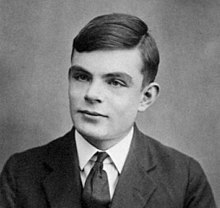
\includegraphics[width=.24\paperwidth]{Figures/AlanTuring}
%			\end{center}
%
%		\end{multicols}
%
%	\end{frame}
%
%%%%%%%%%%%%%%%%%%%%%%%%%%%%%%%%%%%%%%%%%%%%%
%
%	\begin{frame}{Algorithms, Circuits and Gates}
%
%		Computer programs are sequential \textbf{algorithms} often expressed as \textbf{flow charts}, also known as \textbf{circuits}. Along these circuits, the information will be affected by simple logical operations, called \textbf{gates}, as to obtain the required final result.
%
%		\begin{center}
%		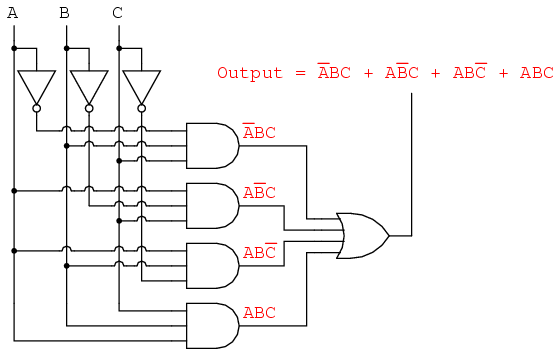
\includegraphics[width=.34\paperwidth]{Figures/Digital_Gates}
%		\end{center}
%
%		\pause
%
%		\vspace{4pt}
%		A digital computer will be able to run any sort of algorithm if this one is encoded using a \textbf{Turing Complete} programming language -- meaning that this language is equivalent to the set of rules used in Turing Machines -- as stated by the CTT.
%
%	\end{frame}
%
%%%%%%%%%%%%%%%%%%%%%%%%%%%%%%%%%%%%%%%%%%%%%
%
%	\begin{frame}{Complexity I}
%
%		Mathematically, a computer program is simply a mapping of an n-bit input to an m-bit output; this can be expressed as:
%
%		\begin{align*}
%			C_{n,m}:\lbrace 0,1 \rbrace^n \rightarrow \lbrace 0,1 \rbrace^m
%		\end{align*}
%
%		Actually since the output is $m$ separate binary registers assembled together, any computer program is built from $m$ mappings of n-bit inputs to a single bit output:
%
%		\begin{align*}
%			C_{n}:\lbrace 0,1 \rbrace^n \rightarrow \lbrace 0,1 \rbrace
%		\end{align*}
%
%		\pause
%
%		Circuit \textbf{complexity} is obviously related to the size of the circuit (the number of gates) and the \textbf{depth} of the circuit, defined as the number of gates traversed in the longest pathway through the circuit.
%
%	\end{frame}
%
%	\begin{frame}{Complexity II}
%
%		\textbf{Computational complexity} is a branch of the theory of computation in theoretical computer science, that focuses on classifying computational problems according to their inherent difficulty, and relating those classes to each other. \pause
%
%		\begin{itemize}
%			\item \textbf{Class P} are problems which can be solved by a computer in Polynomial time; meaning that the amount of steps necessary to solve a problem scales up as a certain exponent of the number of bits in the input \emph{"n"}. (i.e. Find the biggest number from a given array) \pause
%			\item \textbf{Class NP} are problems for which any \underline{given solution} can be checked in polynomial time. (i.e. Sudokus, Prime factorization...) independently of the time it actually takes to solve them $\Rightarrow$ Good problems for \textbf{encryption systems}!
%		\end{itemize}
%
%		\pause
%
%		\vspace{-8pt}
%		\begin{align*}
%			\boldsymbol{P \subseteq NP \quad \Rightarrow \quad P \overset{?}{=} NP \quad } \\
%			\text{\underline{Millenium Prize Problem} 1M\$}
%		\end{align*}
%		\vspace{-20pt}
%
%	\end{frame}
%
%%%%%%%%%%%%%%%%%%%%%%%%%%%%%%%%%%%%%%%%%%%%%
%%%%%%%%%%%%%%%%%%%%%%%%%%%%%%%%%%%%%%%%%%%%%
%
%	\begin{frame}{Information Theory}
%
%		Quantum Information looks at QM from the perspective of trying to determine which are the \textbf{constraints} on how nature conserves certain properties through different processes.
%
%		\begin{multicols}{2}
%
%			The most basic unit of classical-information is called a \textbf{bit}. On the other hand, the most basic unit of quantum-information is called a \textbf{qubit} and it is nothing but the Hilbert space described by a basis of two distinguishable states.
%
%			\columnbreak
%			\begin{center}
%		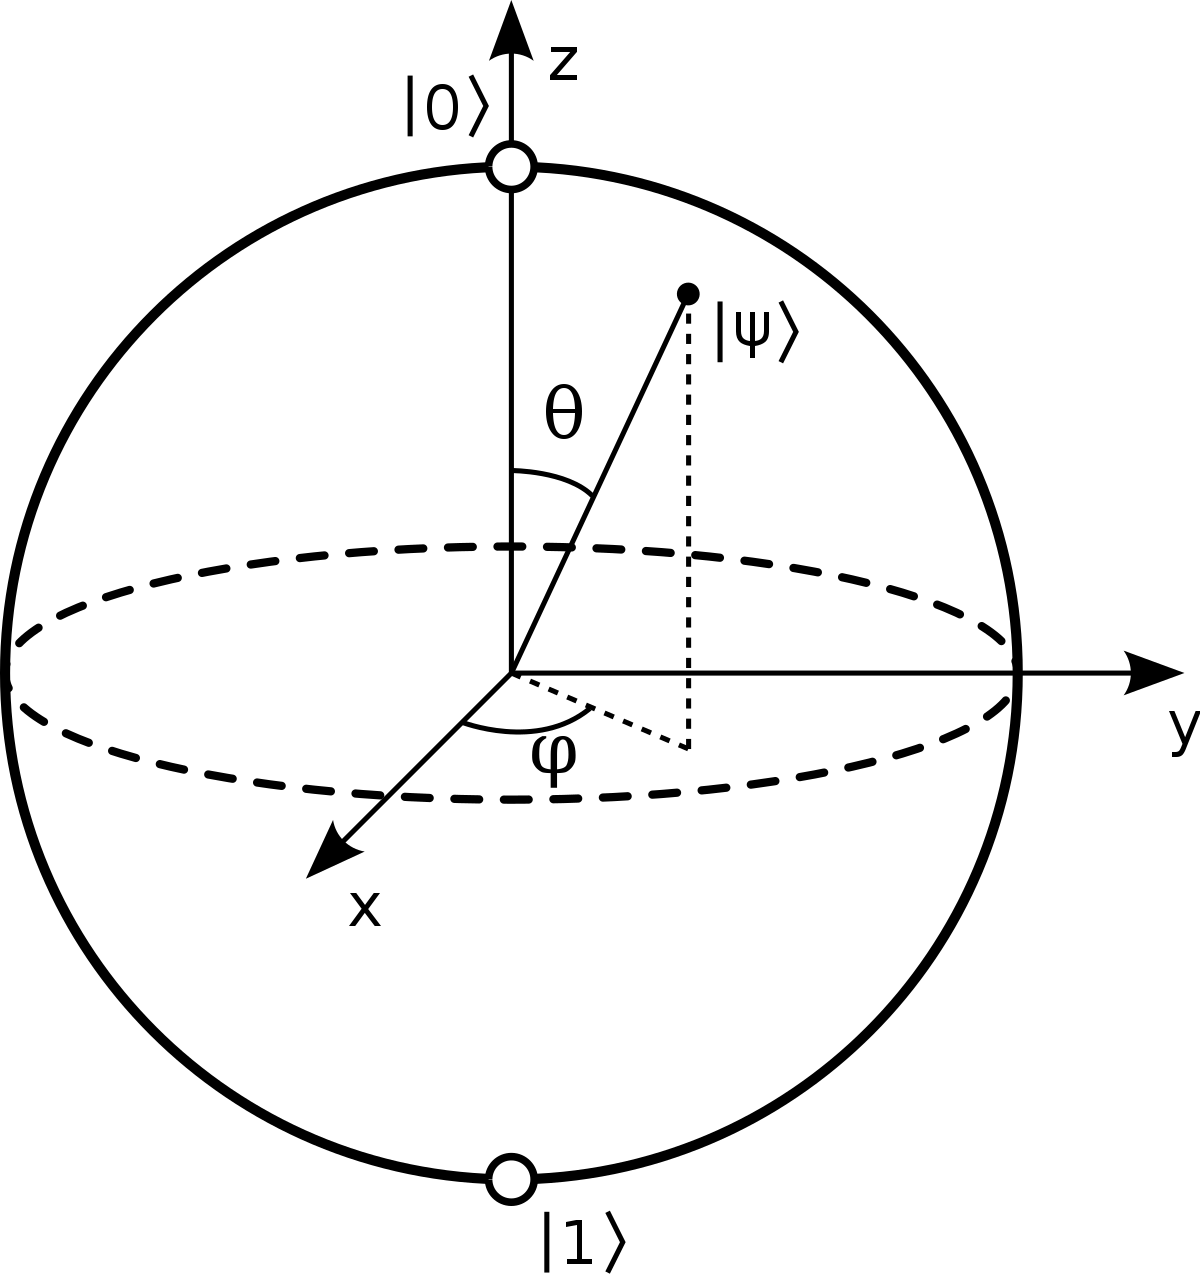
\includegraphics[width=.26\paperwidth]{Figures/Bloch_Sphere}
%			\end{center}
%
%		\end{multicols}
%
%	\end{frame}
%
%%%%%%%%%%%%%%%%%%%%%%%%%%%%%%%%%%%%%%%%%%%%%
%
%	\begin{frame}{Example: Unitary Transformations}
%
%		\textit{\underline{Example:} Preserving information about the distinguishability of two states (Spin-up VS Spin-down) through a transformation, leads to the necessary condition of \textbf{Unitarity}.}
%
%		\begin{align*}
%			&\action<2->{ \braket{0}{1} =0 \quad (\forall t) \quad \& \quad \ket{\Psi (t)} = U\ket{\Psi} } \\
%			 \\
%			&\action<3->{ \braket{0(t)}{1(t)} = \braketop{0}{U^\dagger U}{1} } \action<4->{ \equiv \braket{0}{1}=0 \quad } \action<5->{ \Rightarrow } \\
%			&\action<5->{ \Rightarrow U^\dagger U = \mathbb{I} \quad \mathbb{(Q.E.D.)} }
%		\end{align*}
%
%		\action<6->{
%		From this \textbf{conservation of information} property, it is straight forward to prove that in general $\braket{\Phi}{\Psi}:= \text{const.} (\forall t)$, for any evolution $U$ and any quantum states $\ket{\Psi}$, $\ket{\Phi}$.
%		}
%
%	\end{frame}
%
%%%%%%%%%%%%%%%%%%%%%%%%%%%%%%%%%%%%%%%%%%%%%
%
%	\begin{frame}{No-Cloning Theorem}
%
%		\textbf{Classical information can be copied} at will. The laws of classical physics allow us to look at some information coded in classical states (i.e. orientation of an arrow) and prepare another classical system so that it perfectly resembles the first.
%
%		\begin{multicols}{2}
%
%			If we could \textbf{clone a quantum state}, then by measuring one of the copies we would be able to learn something about the other without disturbing it. So it has to be impossible in the quantum regime.
%
%			\columnbreak
%			\begin{center}
%		
\includegraphics[width=.28\paperwidth]{Figures/clones}
%			\end{center}
%
%		\end{multicols}
%
%	\end{frame}
%
%%%%%%%%%%%%%%%%%%%%%%%%%%%%%%%%%%%%%%%%%%%%%
%
%	\begin{frame}{Formal Proof I}
%
%		To prove this we need to think of what a \textbf{cloning machine} is. It will be an apparatus with two slots $\lbrace A, B \rbrace$, such that in the beginning the quantum states for each slot are $\ket{\Psi}_A$ (the one we want to clone) and $\ket{e}_B$ a generic initialization state. After the process -- which has to be unitary -- we will need to get states $\ket{\Psi}_A$ and $\ket{\Psi}_B$ for each slot. In other words:
%
%		\begin{align*}
%			{ U\ket{\Psi}_A\ket{e}_B = \ket{\Psi}_A\ket{\Psi}_B }
%		\end{align*}
%
%		\pause
%
%		If we now check what happens for another generic state $\ket{\Phi}$, we will again have:
%
%		\begin{align*}
%			{ U\ket{\Phi}_A\ket{e}_B = \ket{\Phi}_A\ket{\Phi}_B }
%		\end{align*}
%
%	\end{frame}
%
%%%%%%%%%%%%%%%%%%%%%%%%%%%%%%%%%%%%%%%%%%%%%
%
%	\begin{frame}{Formal Proof II}
%
%		Taking the inner product of these two equations:
%
%		\begin{align*}
%			&\braket{\Psi}{\Phi} = \bra{\Psi}_A\bra{e}_B\ket{\Phi}_A\ket{e}_B \equiv \bra{\Psi}_A\bra{e}_B U^\dagger U\ket{\Phi}_A\ket{e}_B \\
%			&= \braket{\Psi}{\Phi}\braketop{e}{U^\dagger U}{e} = \braket{\Psi}{\Phi} \braket{\Psi}{\Phi} \Rightarrow \\
%			\action<2->{ \\
%			&\Rightarrow \braket{\Psi}{\Phi} = ( \braket{\Psi}{\Phi} )^2 \Rightarrow
%			\begin{cases}
%				\braket{\Psi}{\Phi} = 0 \\
%				\braket{\Psi}{\Phi} = 1
%			\end{cases} }
%		\end{align*}
%
%		\action<3->{
%		Which means that we can only clone states that form a basis of the corresponding \textit{Hilbert Space} using such unitary transformation $U$. Therefore, \textbf{a single \textit{universal} transformation cannot clone a \textit{general} quantum state}. This is also true for non-unitary transformations.
%		}
%
%		\vspace{8pt}
%		\action<4->{
%		On the other hand, it is straight forward to show in the same manner that \textbf{quantum teleportation} is indeed allowed.
%		}
%
%	\end{frame}
%
%%%%%%%%%%%%%%%%%%%%%%%%%%%%%%%%%%%%%%%%%%%%%
%
%	\begin{frame}{Implications}
%
%		As a matter of fact, there is some deeper reason why this happens. Cloning quantum information will mean \textbf{superluminal communication} (faster than light) and viceversa.
%
%		\begin{multicols}{2}
%			\begin{center}
%		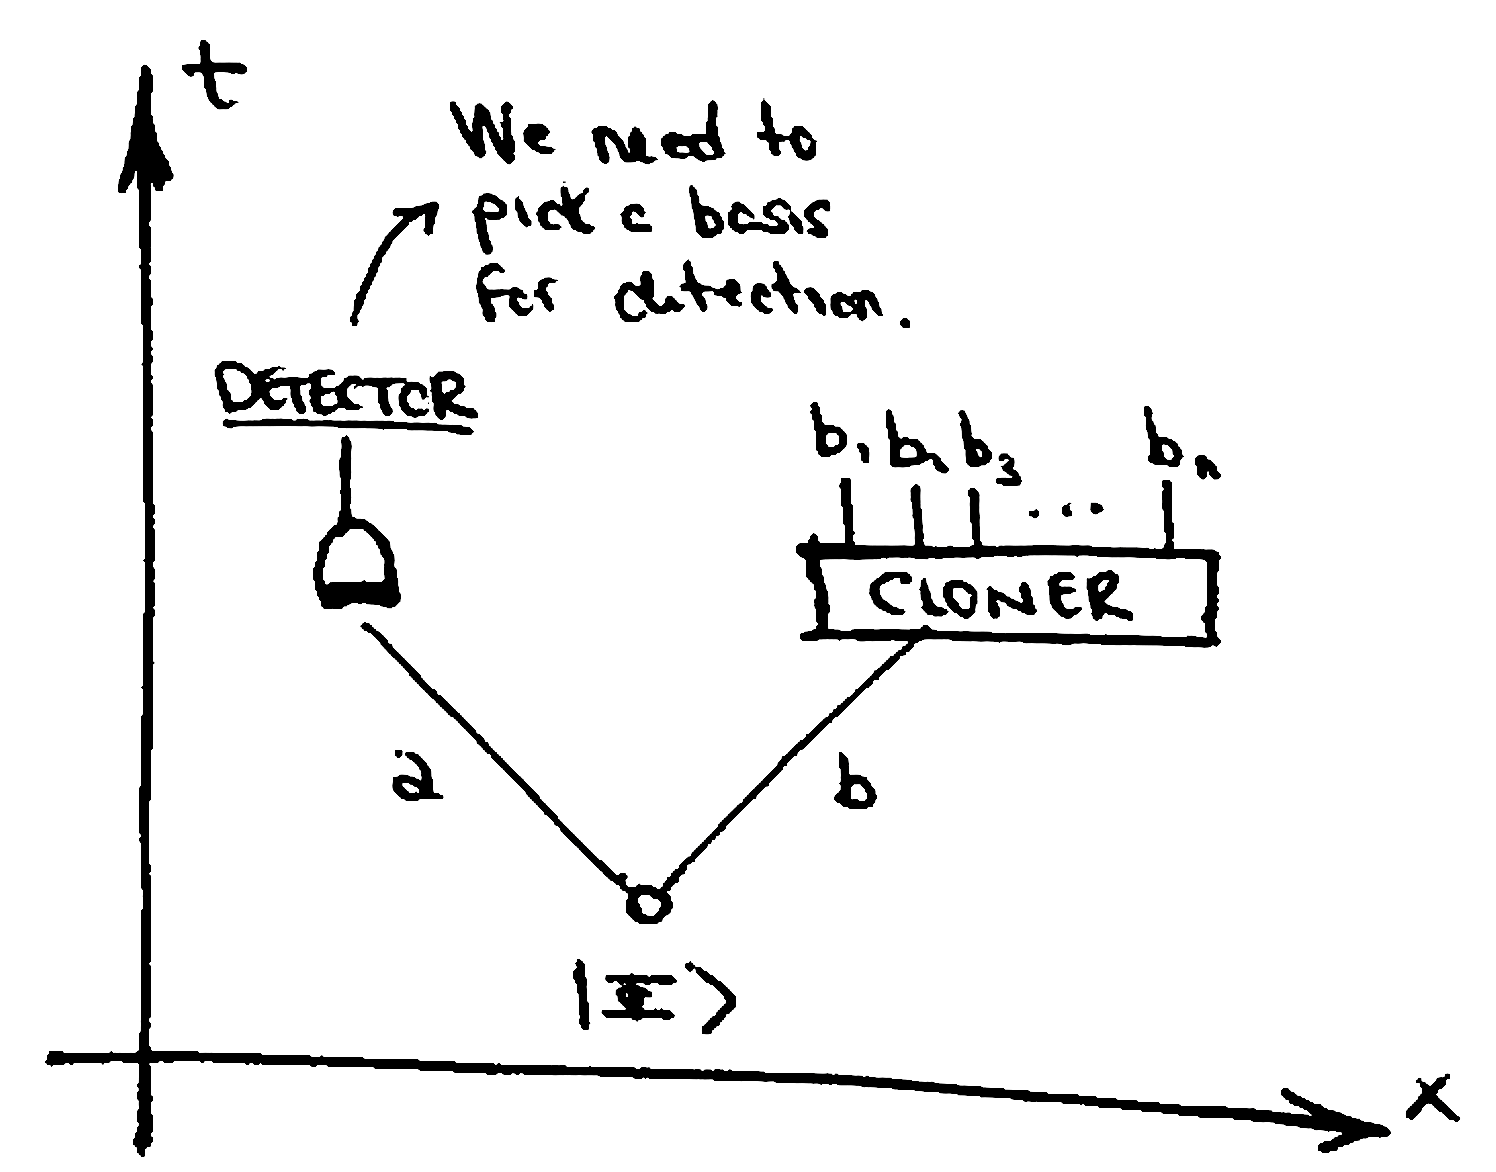
\includegraphics[width=.28\paperwidth]{Figures/Cloning_Superluminal}
%			\end{center}
%			\columnbreak
%			\begin{center}
%		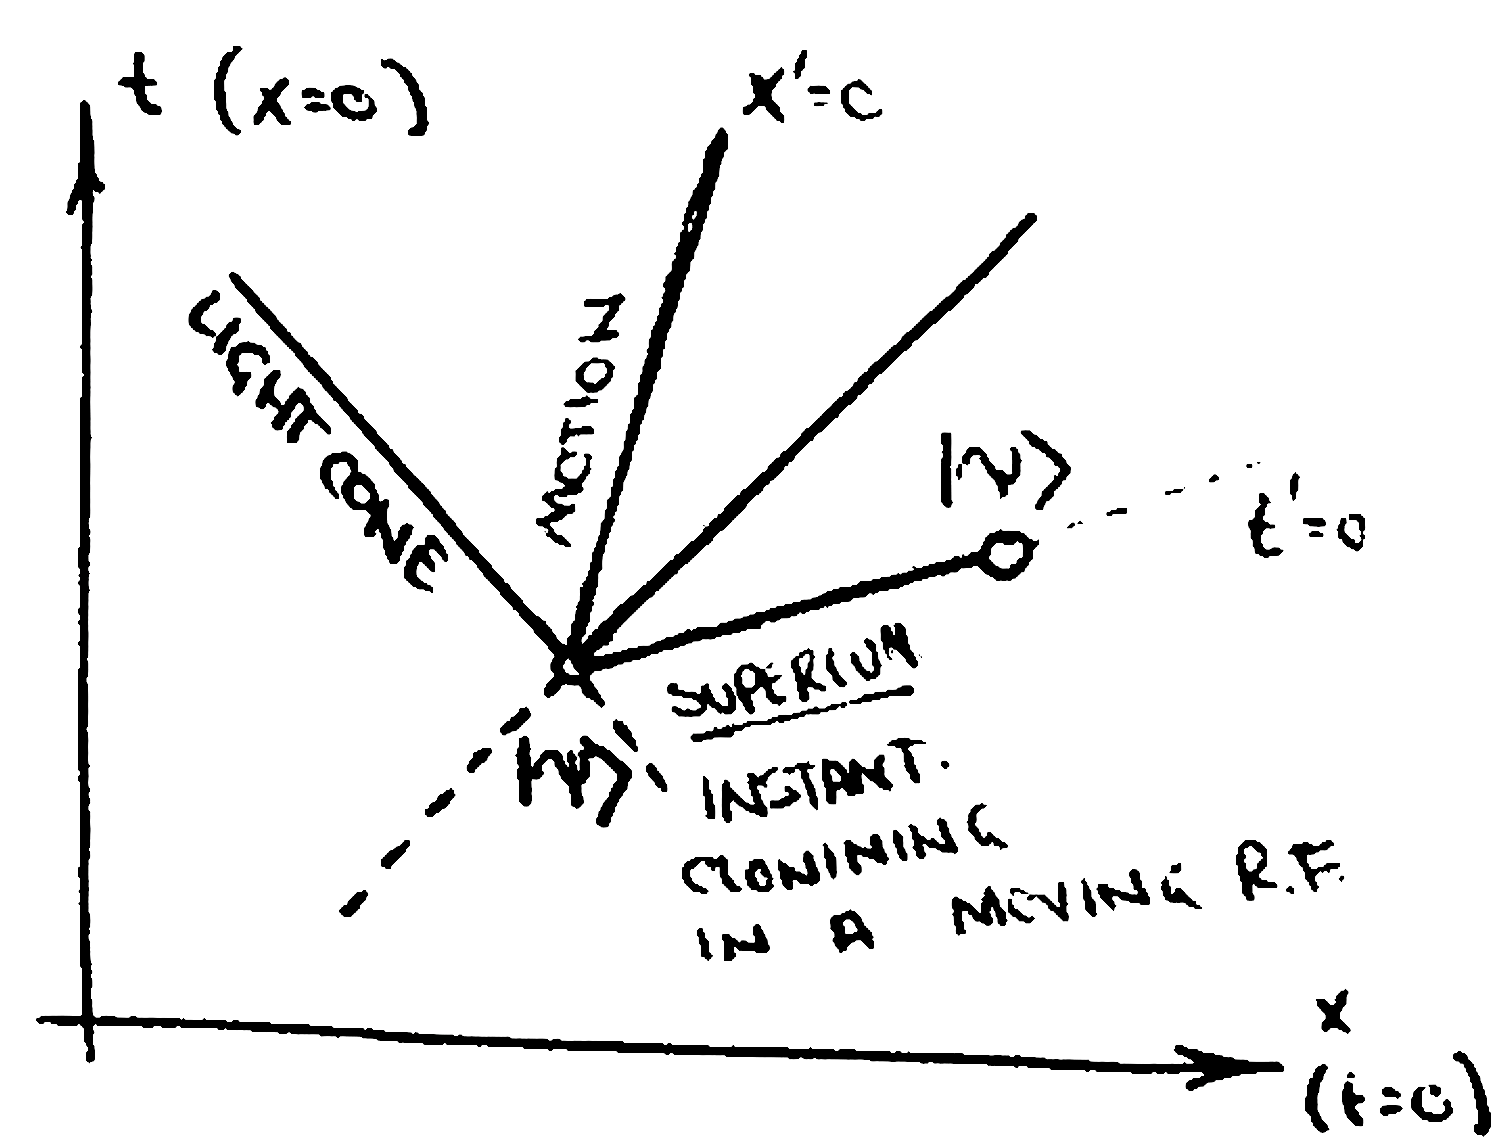
\includegraphics[width=.28\paperwidth]{Figures/Superluminal_Cloning}
%			\end{center}
%		\end{multicols}
%
%		\pause
%
%		\begin{itemize}
%		\item By measuring on different bases we would be able to send a superluminal message. \pause
%		\item In some inertial reference frame, superluminal communication is the same as cloning.
%		\end{itemize}
%
%	\end{frame}
%
%%%%%%%%%%%%%%%%%%%%%%%%%%%%%%%%%%%%%%%%%%%%%
%%%%%%%%%%%%%%%%%%%%%%%%%%%%%%%%%%%%%%%%%%%%%
%
%	\begin{frame}{General-Purpose Quantum Computers}
%
%		For this presentation, we are going to be interested in looking at \textbf{digital quantum computers}, how they work and what kind of applications they have. Some examples of qubits used are:
%
%		\pause
%		\vspace{8pt}
%		\begin{itemize}
%			\item \textbf{Current Loops in superconductors}: $\ket{\circlearrowleft}$ , $\ket{\circlearrowright}$
%			\item \textbf{Polarization}: $\ket{\updownarrow}$ , $\ket{\leftrightarrow}$
%			\item \textbf{Spin}: $\ket{\upharpoonleft}$ , $\ket{\downharpoonleft}$
%			\item \textbf{Energy levels in an atom}: $\ket{\circ}$ , $\ket{\odot}$
%			\item \textbf{Direction of propagation}: $\ket{\uparrow}$ , $\ket{\rightarrow}$
%		\end{itemize}
%
%		\pause
%		\vspace{8pt}
%		Another thing to notice is that \textbf{quantum gates} will only perform unitary transformations, and these transformations will be \textbf{reversible}; unlike classical gates.
%
%	\end{frame}
%
%%%%%%%%%%%%%%%%%%%%%%%%%%%%%%%%%%%%%%%%%%%%%
%
%	\begin{frame}{Hadamard Gate}
%
%		The only, but probably one the most important gates that we want to introduce is the \textbf{Hadamard Gate}. This gate performs a $45º$ rotation followed by a reflection along the $45º$ axis. Intuitively, we will denote the resulting states $\ket{+}$ and $\ket{-}$.
%
%		\action<2->{
%		\begin{center}
%			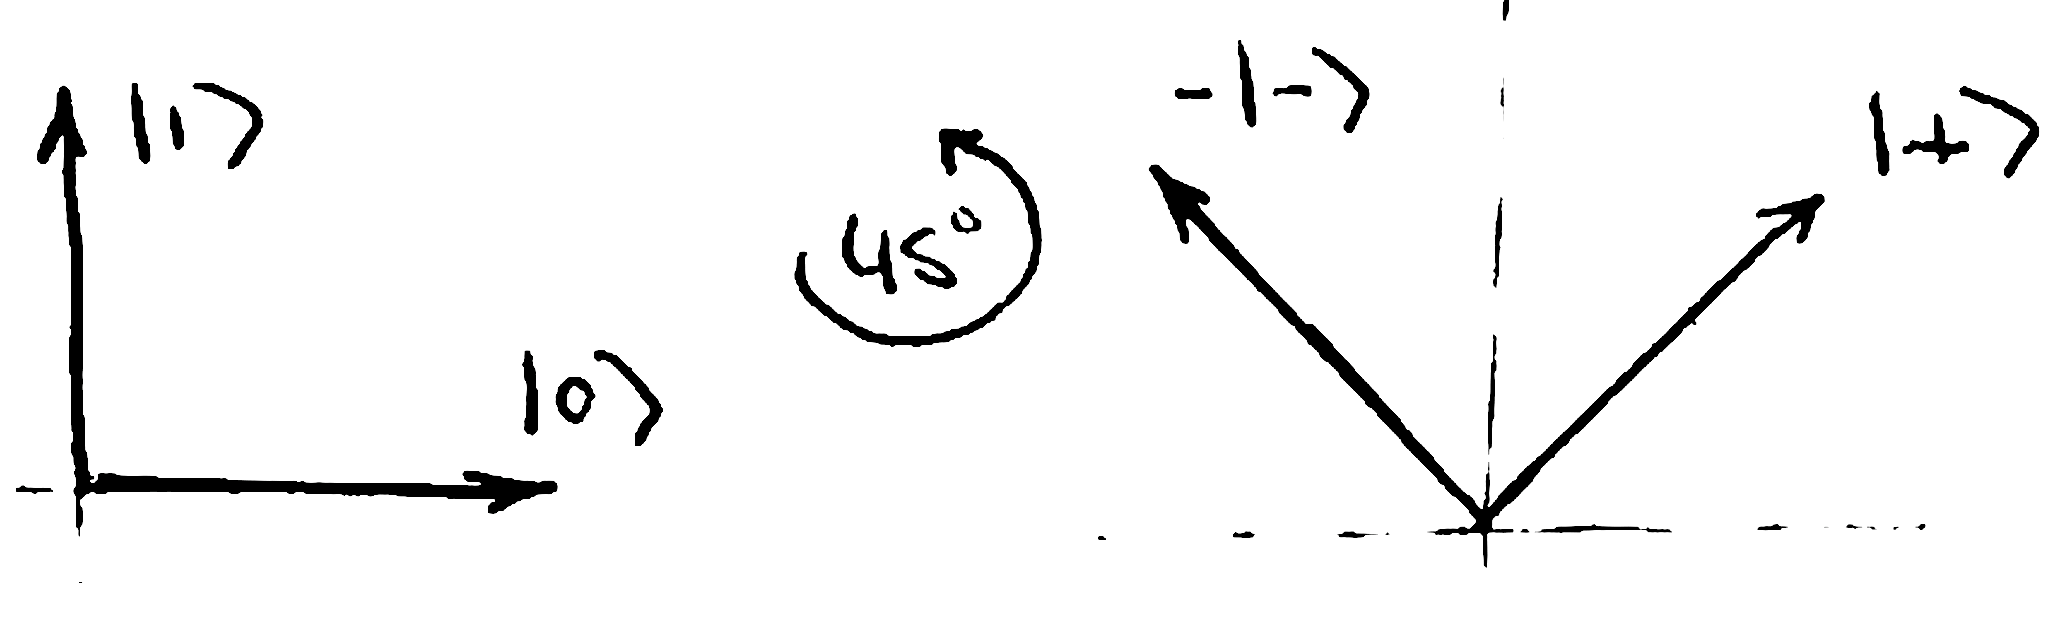
\includegraphics[width=.44\paperwidth]{Figures/Hadamard_Rotation}
%		\end{center}
%		}
%
%		\vspace{-24pt}
%		\begin{multicols}{2}
%			\action<3->{
%			\begin{align*}
%				\hat{\text{H}} &=
%				\underbrace{
%				\begin{bmatrix}
%					0 & 1 \\
%					1 & 0
%				\end{bmatrix}
%				}_{\text{Reflection}}
%				\underbrace{
%				\frac{1}{\sqrt{2}}
%				\begin{bmatrix}
%					1 & -1 \\
%					1 & 1
%				\end{bmatrix}
%				}_{\text{Rotation}} = \\
%				&= \frac{1}{\sqrt{2}}
%				\begin{bmatrix}
%					1 & 1 \\
%					1 & -1
%				\end{bmatrix}
%			\end{align*}
%			}
%			\columnbreak
%			\action<2->{
%			\begin{center}
%				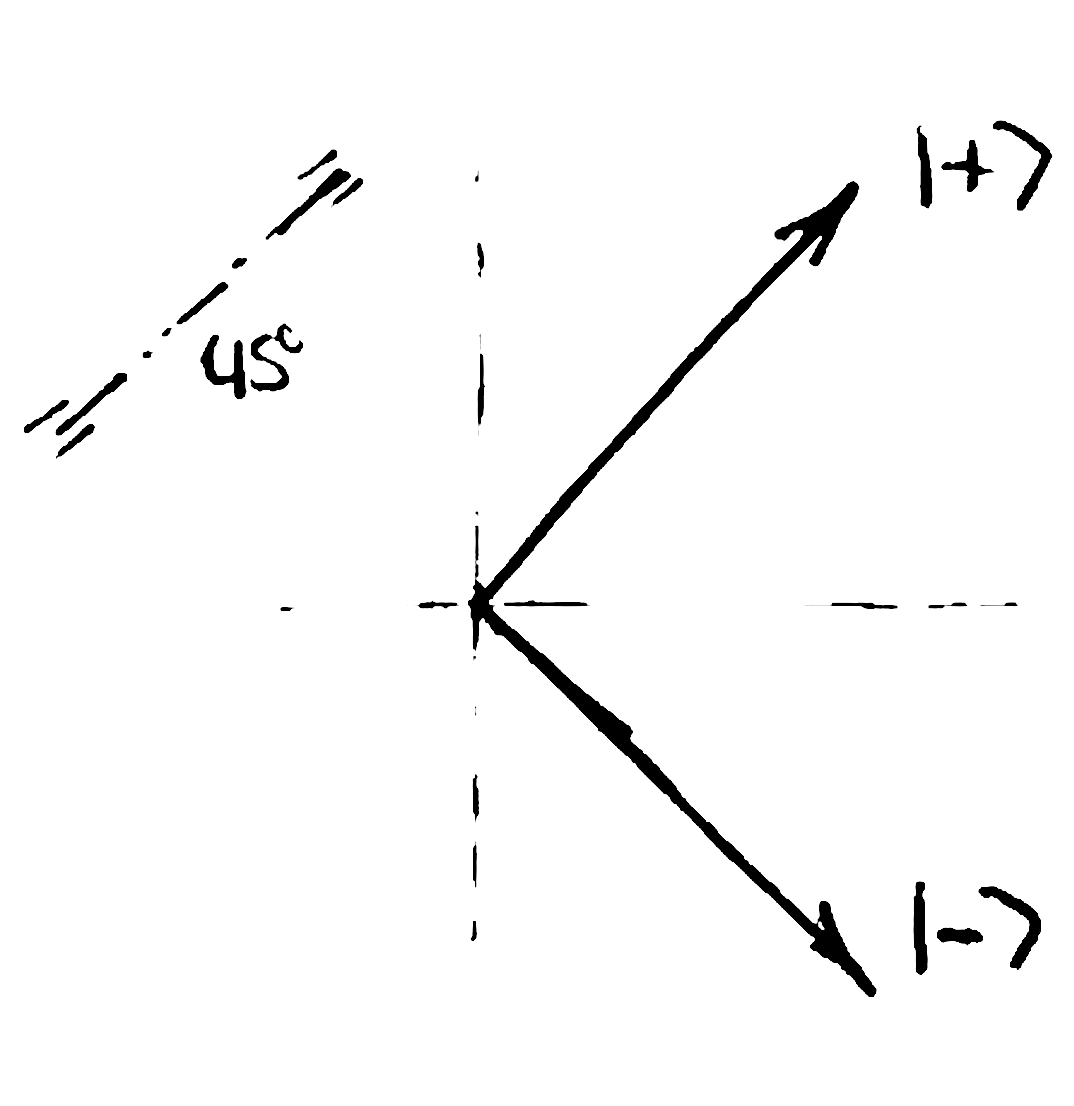
\includegraphics[width=.28\paperwidth]{Figures/Hadamard_Reflection}
%			\end{center}
%			}
%		\end{multicols}
%		\vspace{-28pt}
%
%	\end{frame}
%
%%%%%%%%%%%%%%%%%%%%%%%%%%%%%%%%%%%%%%%%%%%%%
%
%	\begin{frame}{Deutsch’s Problem I}
%
%		Let's try to solve the following problem:
%
%		\vspace{8pt}
%		\textit{"Given a switch and a bulb, which is the most efficient way (fewer operations) of telling whether they are connected or not?"}
%
%		\vspace{8pt}
%		\begin{multicols}{2}
%		\action<2->{\textbf{Classical:}}
%		\begin{enumerate}
%			\item<2-> \label{m1} Look at the states of the bulb and the switch once
%			\item<3-> Change the state of the switch
%			\item<4-> \label{m2} Look at the states of the bulb and the switch again
%			\item<5-> Compare \ref{m1} and \ref{m2}
%		\end{enumerate}
%		\vspace{4pt}
%		\begin{center}
%			\action<6->{\textbf{\underline{2 MEASUREMENTS}}}
%		\end{center}
%
%		\columnbreak
%		\begin{center}
%			
\includegraphics[width=.20\paperwidth]{Figures/Light_Bulb} \\
%			
\includegraphics[width=.08\paperwidth]{Figures/Switch_ON} \\
%			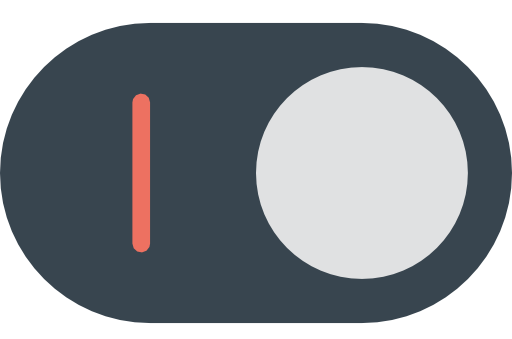
\includegraphics[width=.08\paperwidth]{Figures/Switch_OFF}
%		\end{center}
%		\end{multicols}
%
%	\end{frame}
%
%	%%%%%%%%%%%%%%%%%%%%%%%%%%%%%%%%%%%%%%%%%%%%
%
%	\begin{frame}{Deutsch’s Problem II}
%
%		\textbf{Quantum:} \\
%		We need to express the problem in a more mathematical way in order to tackle it.
%
%		\vspace{-6pt}
%		\begin{align*}
%			& f:\lbrace 0,1 \rbrace \rightarrow \lbrace 0,1 \rbrace \quad \Rightarrow \quad \underbrace{f(0)\neq f(1)}_{\text{Connected}}? \\
%			& \ket{x} \rightarrow \boxed{\text{\textbf{Switch}}} \rightarrow (-1)^{f(x)}\ket{x} \\
%		\end{align*}
%
%		\action<2->{
%		\vspace{-14pt}
%		Let's now try to use \textbf{superposition} to our advantage by introducing the Hadamard Gate:
%		}
%
%		\begin{align*}
%			\action<2->{ \ket{0} \rightarrow \boxed{\hat{\text{H}}} \rightarrow \ket{+} }
%			\action<3->{ \rightarrow \boxed{\text{\textbf{Switch}}} \rightarrow
%			\begin{Bmatrix}
%				\pm \ket{+} \\
%				\pm \ket{-}
%			\end{Bmatrix} }
%			\action<4->{ \rightarrow \boxed{\hat{\text{H}}} \rightarrow
%			\begin{Bmatrix}
%				\pm \ket{0} \\
%				\pm \ket{1}
%			\end{Bmatrix} }
%		\end{align*}
%
%		\vspace{-8pt}
%		\begin{center}
%			\action<5->{
%			\alert{\textbf{\underline{ONLY ONE MEASUREMENT}}} \\
%			{\small Reduction: $2 \rightarrow \log_2(2)=1$ }
%			}
%		\end{center}
%		\vspace{-14pt}
%
%	\end{frame}
%
%%%%%%%%%%%%%%%%%%%%%%%%%%%%%%%%%%%%%%%%%%%%%
%
%	\begin{frame}{Grandiose Interpretation: Period Finding}
%
%		It is difficult to see this right away from the example because of the reduced amount of possible states we are considering, but what we are truly doing is \textbf{finding the periodicity} of the the function $f(x)$ such that $f(x+T) = f(x)$. \\
%
%		\pause
%
%		\vspace{8pt}
%		Because we only have two possible states, it is easier to see it using \textbf{binary arithmetic}:
%
%		\begin{align*}
%		\begin{cases}
%			0 + 0 = 0 \quad & \text{(even)} \\
%			0 + 1 = 1 + 0 = 1 \quad & \text{(odd)} \\
%			1 + 1 = 0 \rightarrow 10 \quad & \text{(even)}
%		\end{cases}
%		\end{align*}
%
%		\pause
%
%		Therefore:
%
%		\begin{align*}
%		\text{If  }
%		\begin{Bmatrix}
%			f(0) \neq f(1) \quad \Rightarrow f(x) = f(x+0) \\
%			f(0) = f(1) \quad \Rightarrow f(x) = f(x+1)
%		\end{Bmatrix}
%		\Rightarrow \text{Periodicities } \lbrace 0,1 \rbrace
%		\end{align*}
%		\vspace{-20pt}
%
%	\end{frame}
%
%%%%%%%%%%%%%%%%%%%%%%%%%%%%%%%%%%%%%%%%%%%%%
%
%	\begin{frame}{Prime Factorization}
%
%		Prime factorization is thought to be a problem in the NP class. Checking a given answer is trivial, but performing the task \textbf{scales exponentially in time} with the size of the input -- at least using the best algorithm we have yet encountered: \textbf{Fast Fourier Transform (FFT)}. \\
%
%		\pause
%
%		\vspace{-12pt}
%		\textit{
%		\begin{small}
%		\begin{multicols}{2}
%			\begin{itemize}
%				\item For any given number $M$ such that $2^{n-1} \leq M \leq 2^n = N$
%				\item FFT splits M into its even/odd subproblems
%				\item Repeats the same with the subproblems until it is left with $N$ single elements
%				\item Recombines
%			\end{itemize}
%			\columnbreak
%			\begin{center}
%				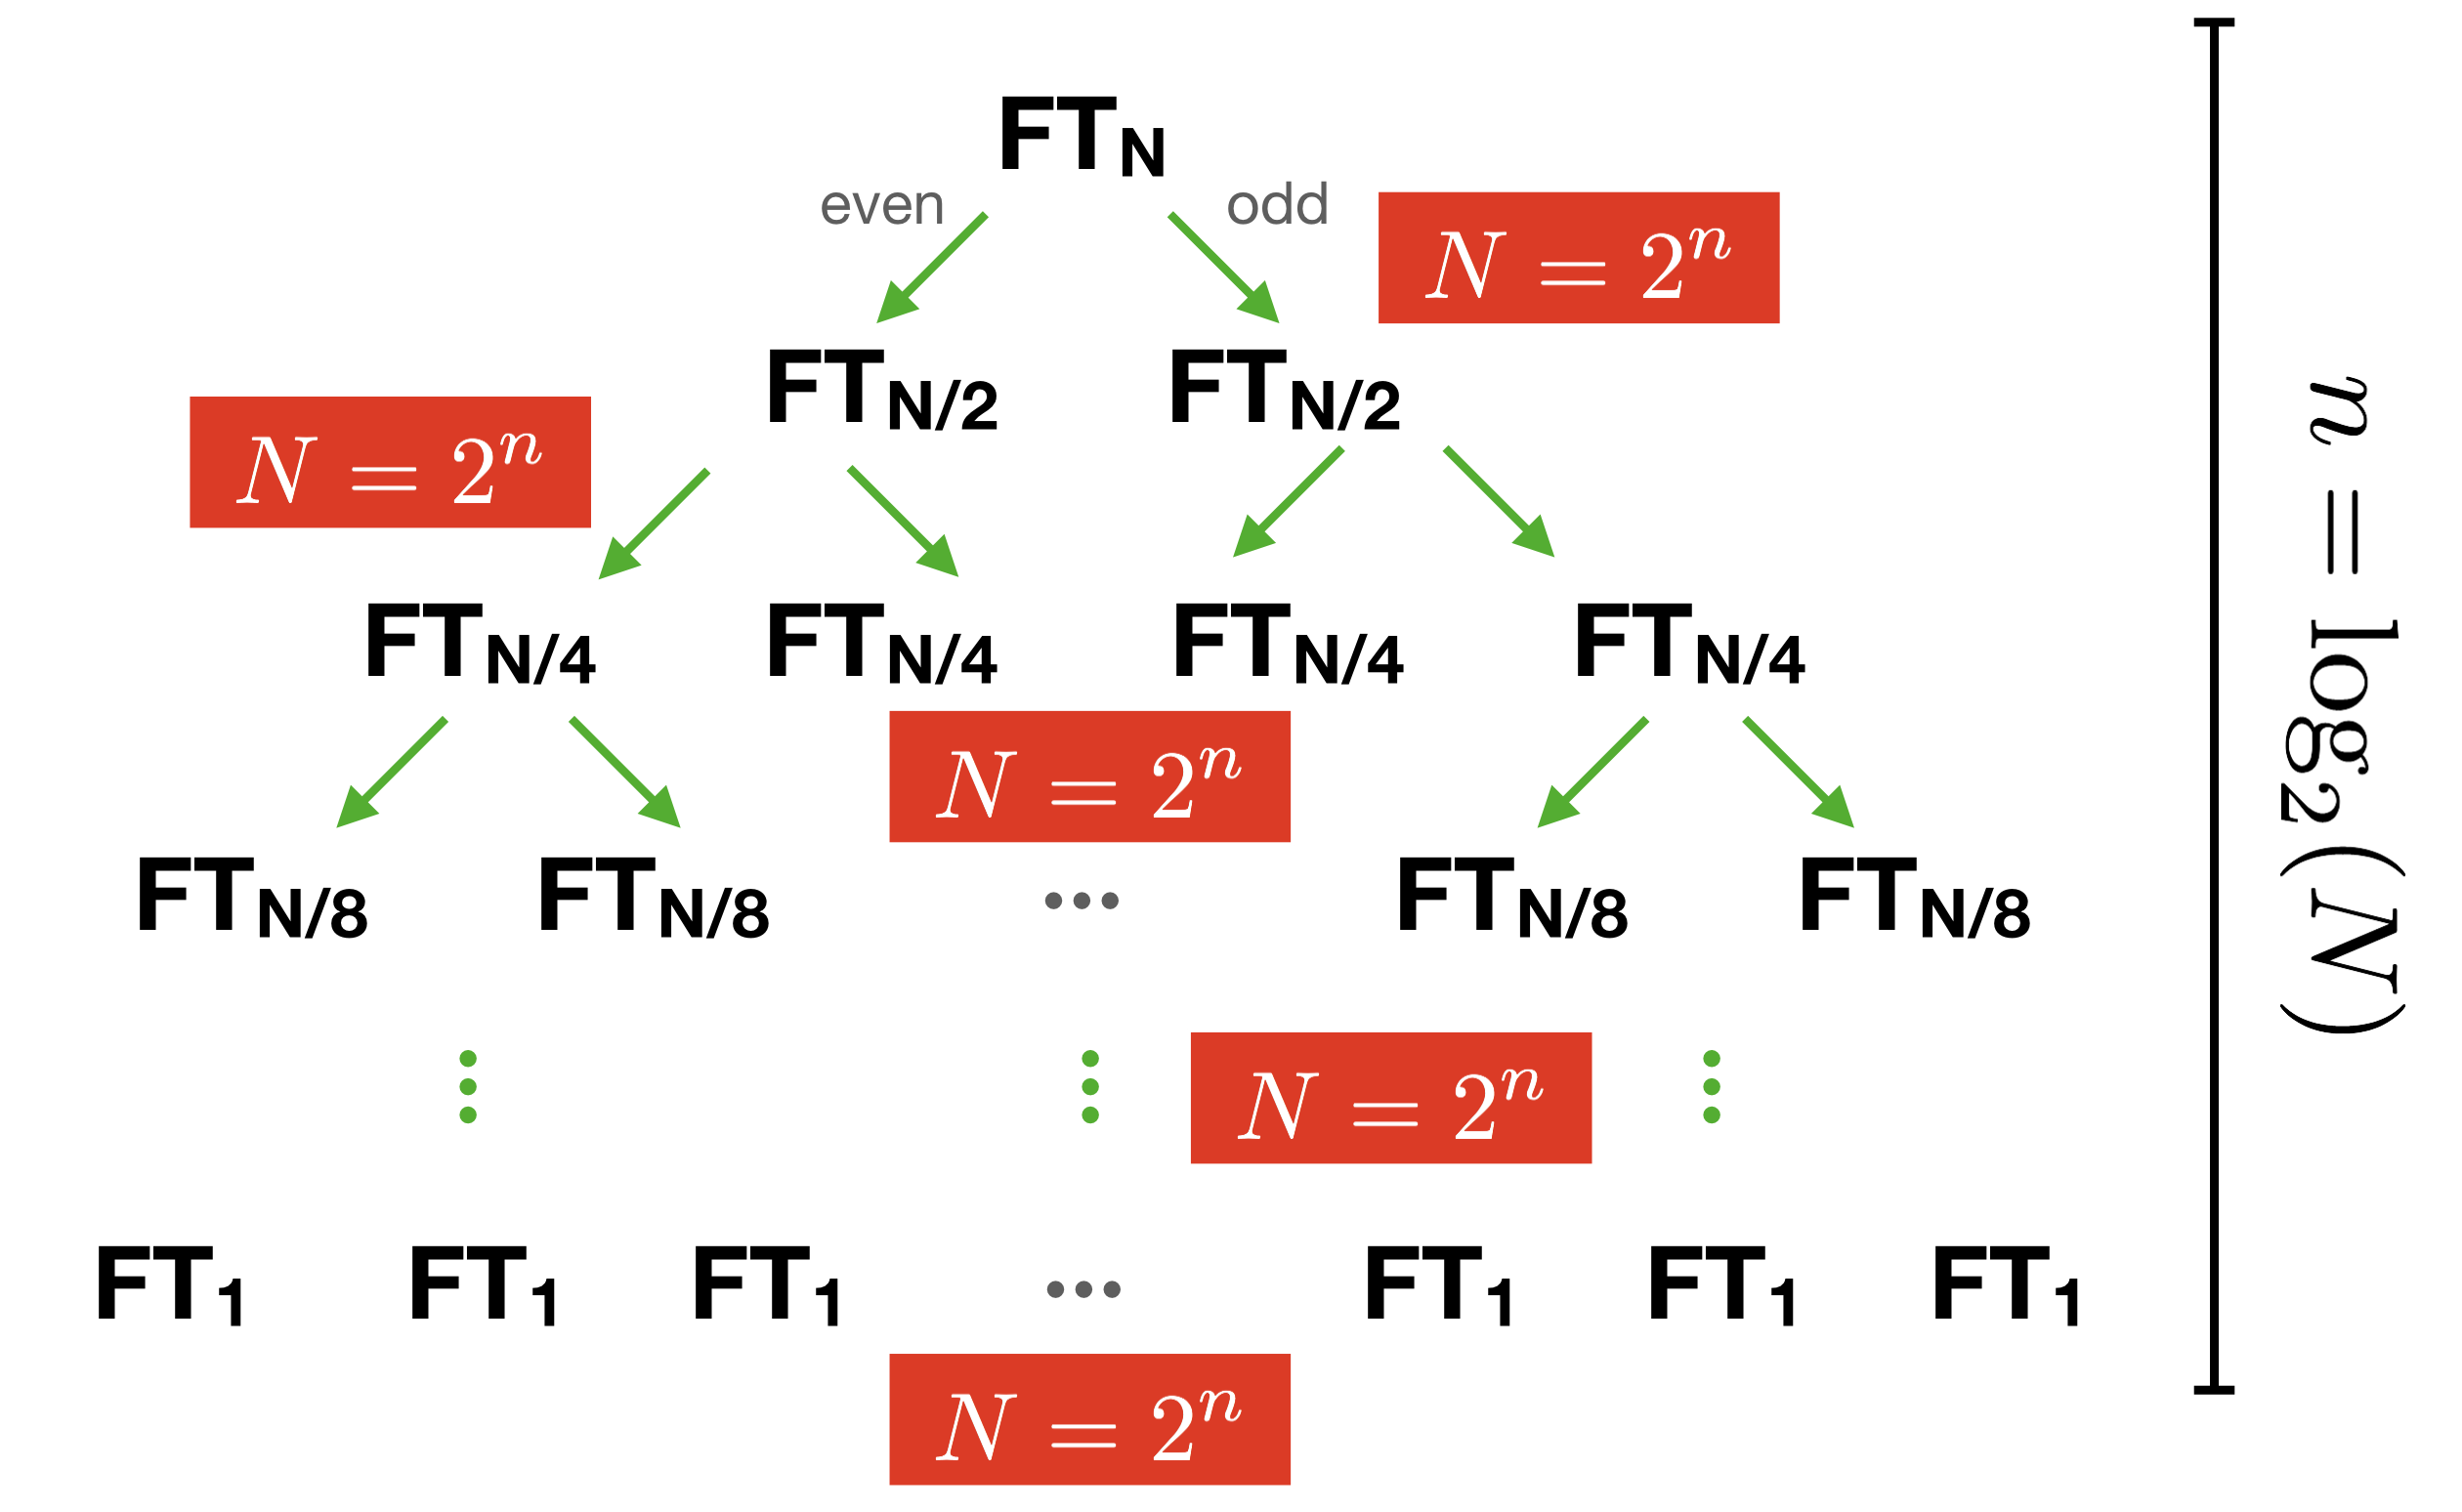
\includegraphics[width=0.40\paperwidth]{Figures/FFT}
%			\end{center}
%		\end{multicols}
%		\end{small}
%		}
%
%		\pause
%
%		\vspace{-8pt}
%		\begin{center}
%			\alert{\textbf{\underline{\#OPERATIONS: $n \cdot N=n \cdot 2^n$}}}
%		\end{center}
%		\vspace{-10pt}
%
%	\end{frame}
%
%%%%%%%%%%%%%%%%%%%%%%%%%%%%%%%%%%%%%%%%%%%%%
%
%	\begin{frame}{Shor's Algorithm}
%
%		MIT Professor \textbf{Peter Shor} came up with a quantum algorithm which, similar to what happened in the \textit{Deutsch's Problem}, makes use of superposition to calculate and recombine all the different subproblems in the FFT, reducing the operational cost of each level from $N \rightarrow \log_2(N)=n$.
%
%		\vspace{-10pt}
%		\begin{center}
%			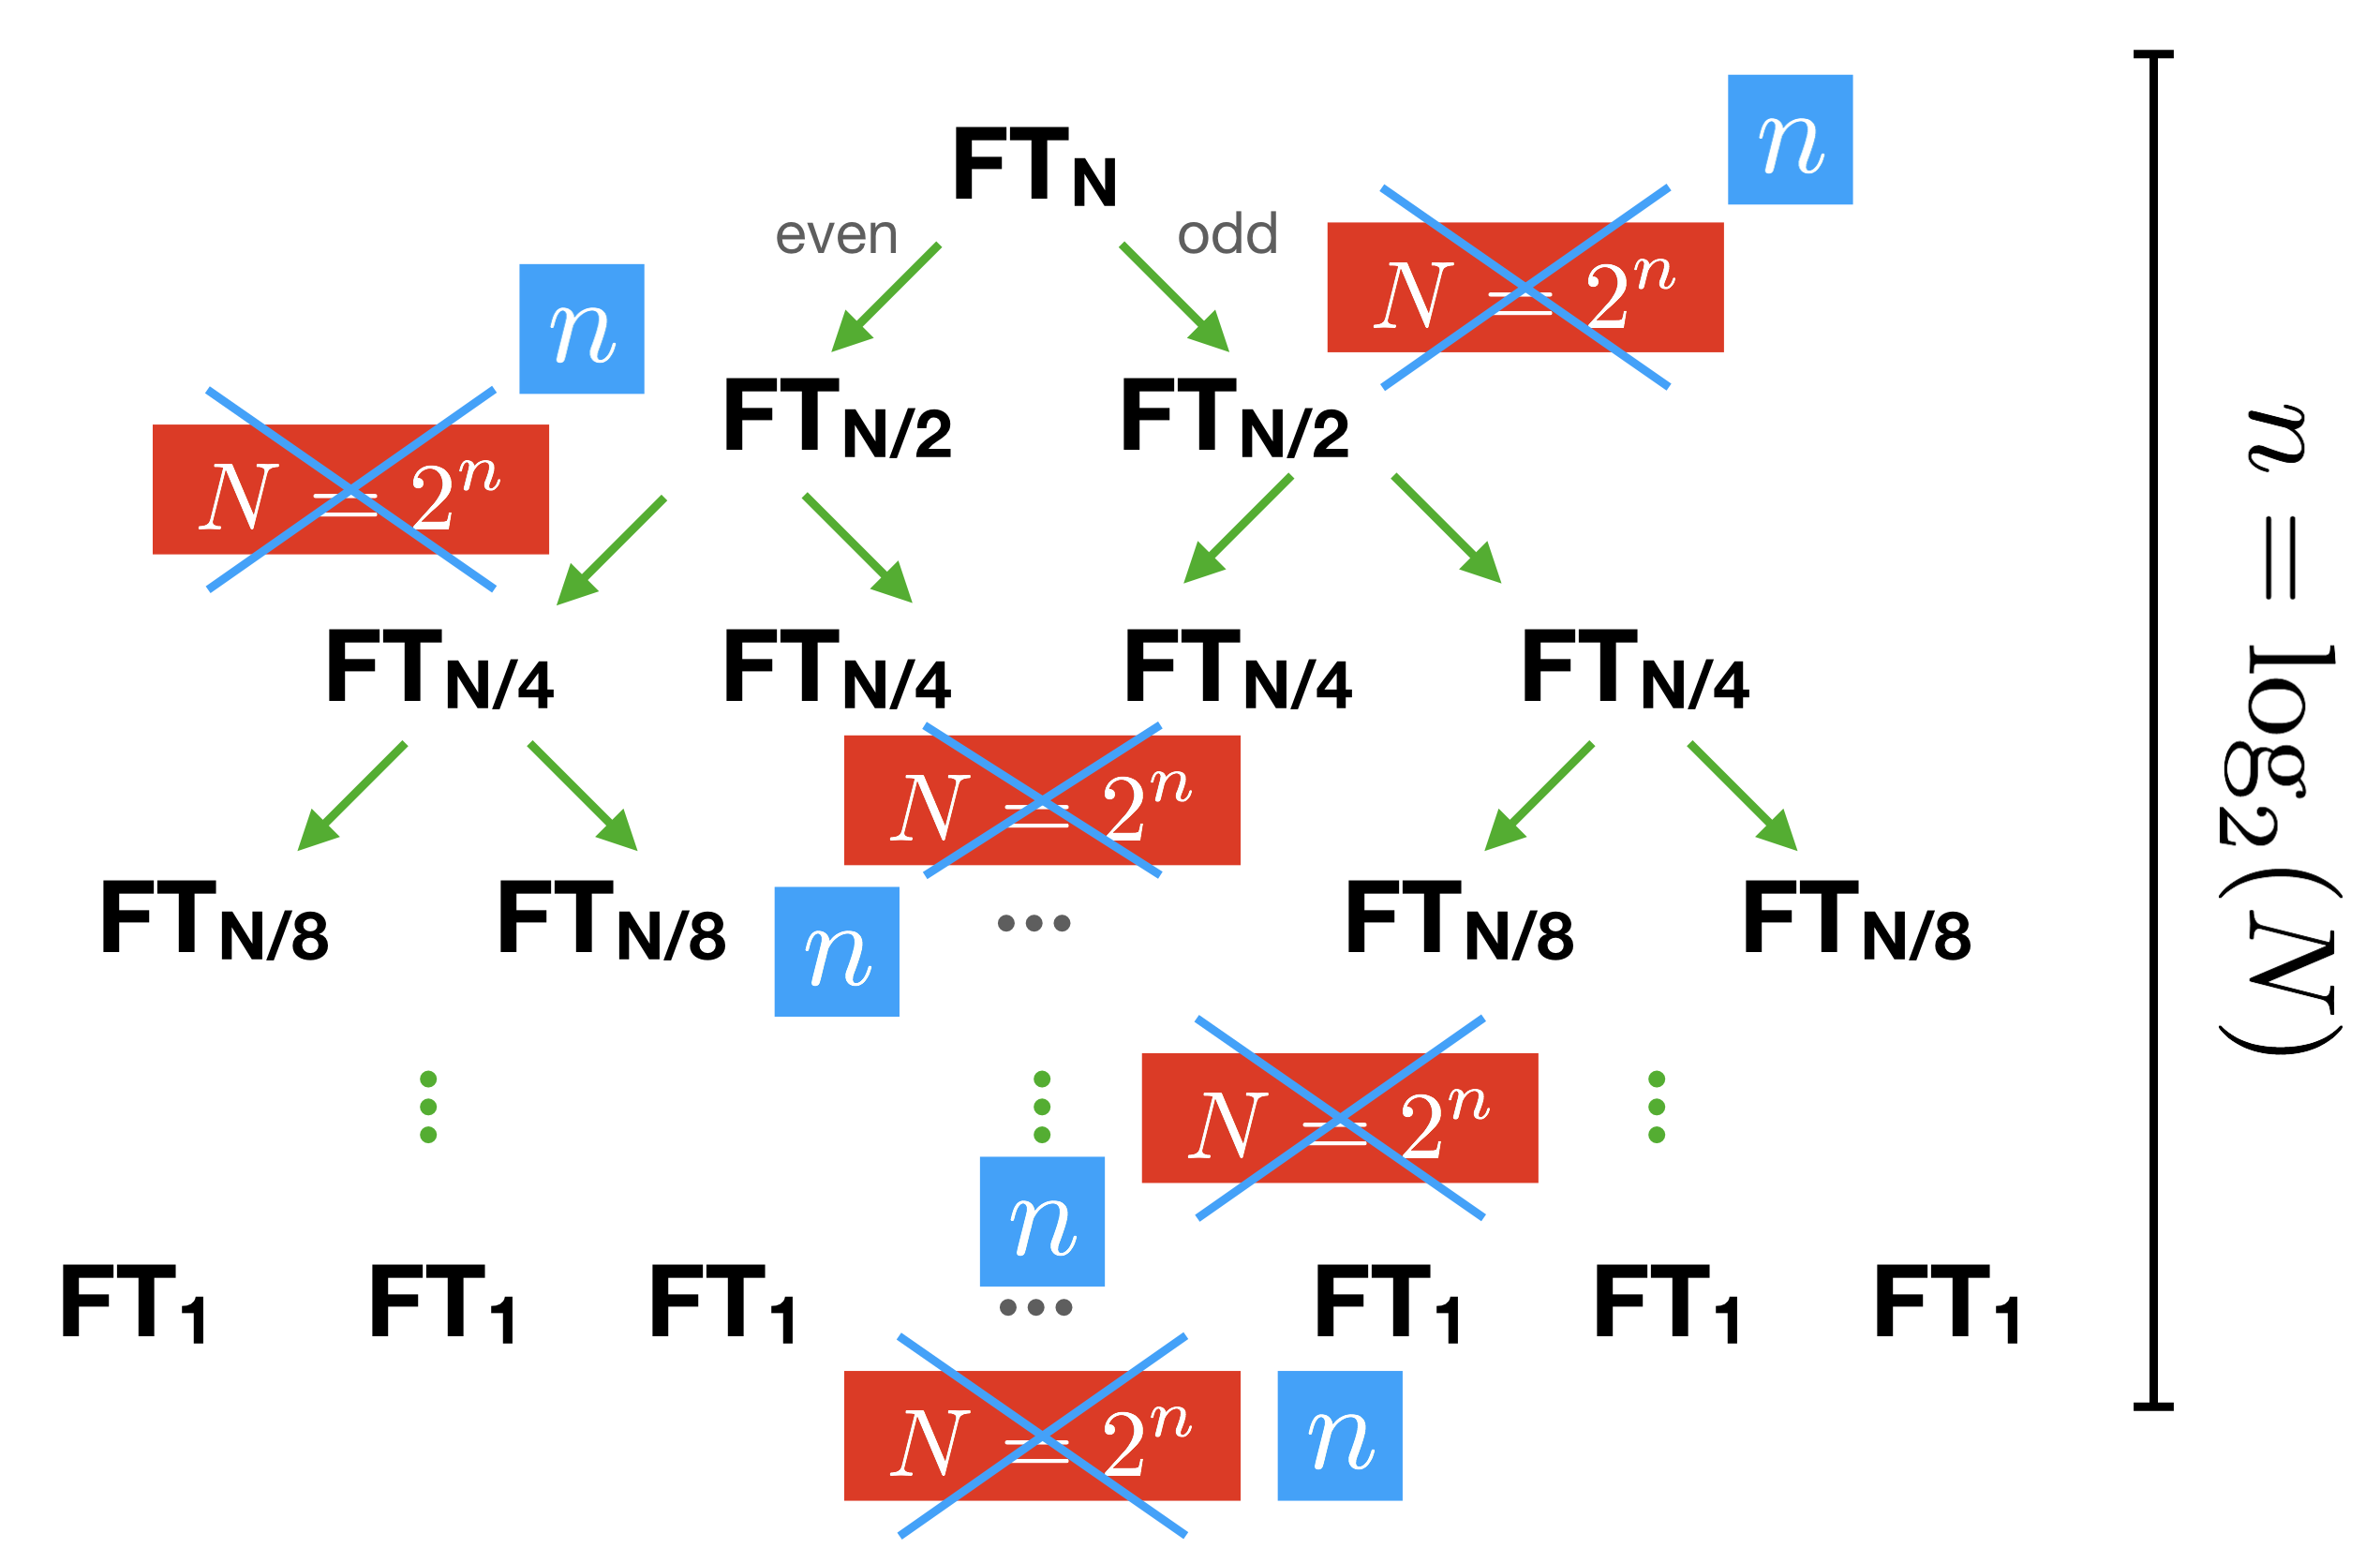
\includegraphics[width=0.46\paperwidth]{Figures/Q_FFT}
%		\end{center}
%
%		\pause
%
%		\vspace{-14pt}
%		\begin{center}
%			\alert{\textbf{\underline{\#OPERATIONS: $n \cdot n = n^2$}}} \\
%			{\small Prime Factorization: \textbf{NP} $\rightarrow$ \textbf{P} }
%		\end{center}
%		\vspace{-10pt}
%
%	\end{frame}
%
%%%%%%%%%%%%%%%%%%%%%%%%%%%%%%%%%%%%%%%%%%%%%
%
%	\begin{frame}{C.T.T. Challenge}
%
%	\action<1->{
%		\alert{
%		\textbf{\underline{Question:}} \textit{Does the Church-Turing Thesis extend to Quantum Computers?} In other other words, are all problems solvable by quantum computers also solvable by Turing machines? Given unlimited time and memory.
%		}
%	}
%
%	\action<2->{
%		\vspace{8pt}
%		\textbf{\underline{My current take:}} \textbf{YES}. As far as one can capture any logical statement on a Turing machine (more or less efficiently), and as far as we have been able to understand quantum mechanics logically (describing them with mathematics) we don’t know yet of any problem which a Turing machine cannot compute. \\
%	}
%	\action<3->{
%		\vspace{4pt}
%		A Quantum Computer can only compute things much more efficiently. Nevertheless, things like entanglement cannot be locally reproduced by a Turing machine \textbf{(Bell’s Theorem)}, although it can be globally described, and so the question is \underline{still unanswered}.
%	}
%
%	\end{frame}
%
%%%%%%%%%%%%%%%%%%%%%%%%%%%%%%%%%%%%%%%%%%%%%
%
%	\begin{frame}{Error Correction: Motivations}
%
%		Because of things like noise, we cannot expect to build qubits in a perfect and ideal way. We will have to account for the possible arising of \textbf{errors}. \\
%
%		\vspace{8pt}
%		 For this reason we distinguish between:
%		\begin{itemize}
%		 \item \textbf{Logical Qubits} $(\# \equiv L)$
%		 \item \textbf{Physical Qubits} $(\# \equiv P > L)$
%		\end{itemize}
%
%		\pause
%
%		\vspace{8pt}
%		This is the main issue that Quantum Computation presents today, as errors spoil the robustness of the more simple computation techniques. Nevertheless, it has been proven that errors $\lesssim 0.01\%$ can be corrected using software and \textbf{quantum error-correction techniques} in order to obtain \textit{Full Quantum Computation}. This is called the \textbf{Fault-Tolerance Theorem}.
%
%	\end{frame}
%
%%%%%%%%%%%%%%%%%%%%%%%%%%%%%%%%%%%%%%%%%%%%%
%
%	\begin{frame}{Error Correction: Simple Method}
%
%		Let's write down some very simple error-correction techniques: \\
%
%		\vspace{10pt}
%		\textbf{Classical:} \\
%		\vspace{-10pt}
%		\begin{align*}
%		\text{Substitute:  }
%		\begin{cases}
%			\lbrace 0 \rbrace \rightarrow \lbrace 0 \rbrace \lbrace 0 \rbrace \lbrace 0 \rbrace \\
%			\lbrace 1 \rbrace \rightarrow \lbrace 1 \rbrace \lbrace 1 \rbrace \lbrace 1 \rbrace
%		\end{cases}
%		\end{align*}
%
%		\pause
%
%		\textbf{Quantum:} (No-Cloning, measurement disturbs, not discrete...) \\
%		\vspace{-4pt}
%		\begin{align*}
%		\text{Entangled \textbf{qutrits}:  }
%		\begin{cases}
%			\ket{0} \rightarrow \ket{0,0,0} + \ket{1,1,1} + \ket{2,2,2} \\
%			\ket{1} \rightarrow \ket{0,1,2} + \ket{1,2,0} + \ket{2,0,1} \\
%			\ket{2} \rightarrow \ket{0,2,1} + \ket{1,0,2} + \ket{2,1,0}
%		\end{cases}
%		\end{align*}
%
%		\vspace{-0pt}
%		Any single qutrit in the entangled picture has the exact same $1/3$ probability of being either $\lbrace 0,1,2 \rbrace$; no matter which original qutrit it corresponds to. Therefore, loosing one will not give out any information and our system will be secured from measurement disturbances. \textbf{Information is encoded in the entanglement}.
%
%	\end{frame}
%
%%%%%%%%%%%%%%%%%%%%%%%%%%%%%%%%%%%%%%%%%%%%%
%%%%%%%%%%%%%%%%%%%%%%%%%%%%%%%%%%%%%%%%%%%%%
%
%	\begin{frame}{Applications: Brief List}
%
%		Some of the foreseeable applications of Quantum Computation which will have a revolutionary impact on society are:
%
%		\begin{multicols}{2}
%			\begin{itemize}
%				\item<2->{ Cryptography }
%				\item<3->{ Optimization Problems }
%				\item<4->{ Pattern Matching }
%				\item<4->{ Data Analysis }
%				\item<5->{ Deep Learning }
%				\item<5->{ Random Sampling Techniques }
%				\item<6->{ Quantum Simulations }
%				\item<6->{ Chemistry Simulations }
%				\item<6->{ Biology Simulations }
%			\end{itemize}
%
%			\columnbreak
%			\action<1->{
%			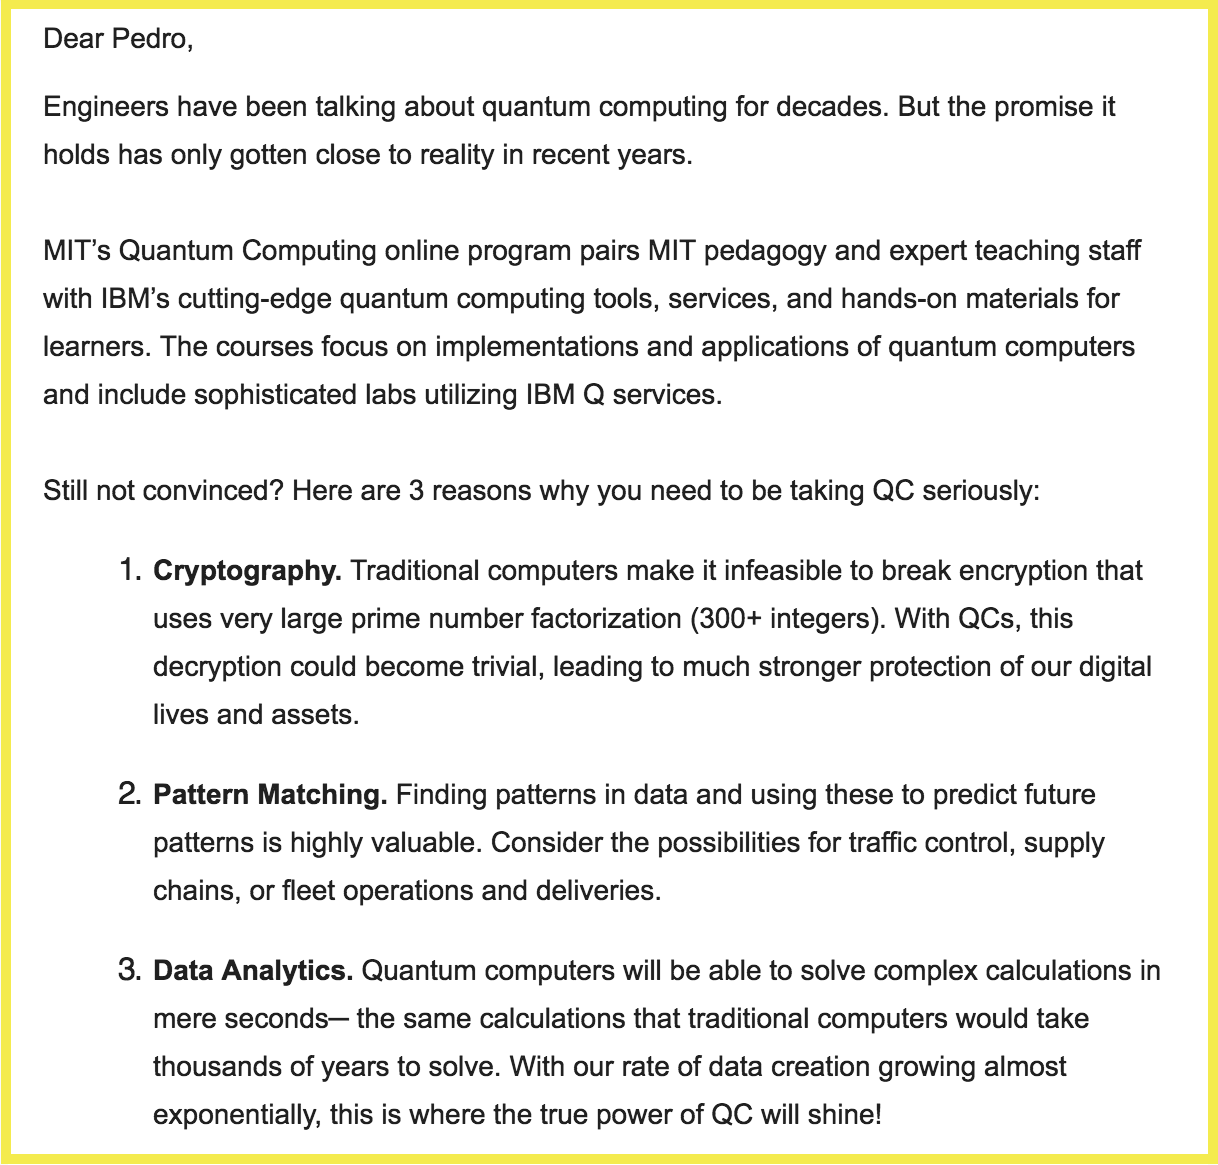
\includegraphics[width=0.38\paperwidth]{Figures/MIT_email} }
%		\end{multicols}
%
%	\end{frame}
%
%%%%%%%%%%%%%%%%%%%%%%%%%%%%%%%%%%%%%%%%%%%%%
%
%	\begin{frame}{Quantum Gravity}
%
%		Some important historical facts to know are:
%		\begin{itemize}
%			\item \textbf{Stephen Hawking} $\rightarrow$ Blackhole entropy (information) is proportional to its surface
%			\item \textbf{Leonard Susskind} $\rightarrow$ Extended this notion to the Holographic Principle $\Rightarrow$ \underline{Q-gravity} emerges on the new dim.
%		\end{itemize}
%
%		\pause
%
%		\begin{multicols}{2}
%			The closer the system is to the projecting surface, the smaller the area it will take to encode all of its information. \\
%			If it is in the exact center, the information gets distributed as in the quantum error-correcting technique we described, making information about gravity well encoded and protected.
%			\columnbreak
%			\begin{center}
%				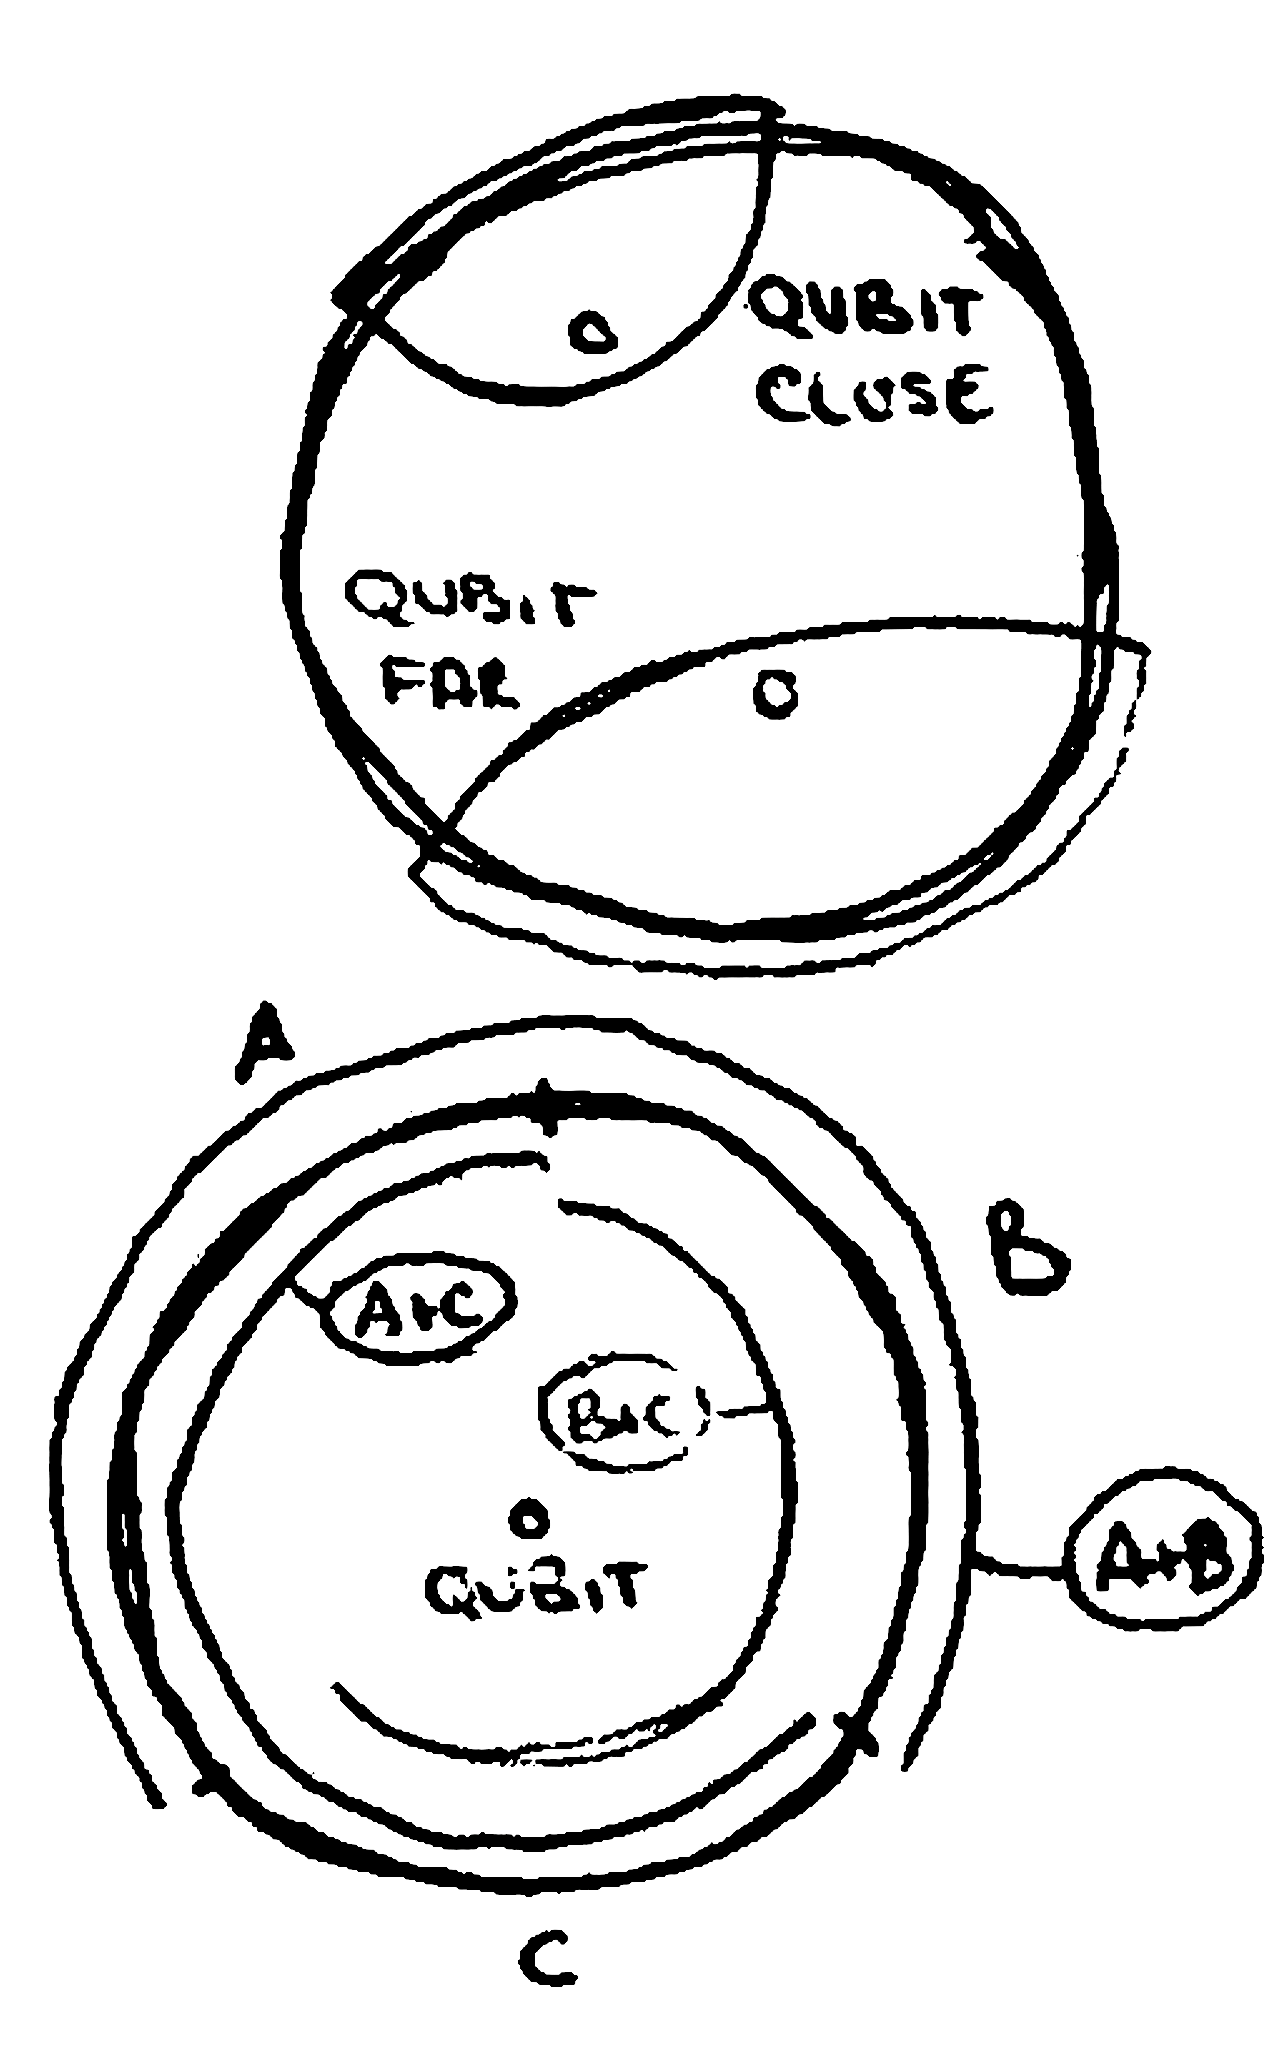
\includegraphics[width=0.24\paperwidth]{Figures/Holographic}
%			\end{center}
%		\end{multicols}
%		\vspace{-20pt}
%
%	\end{frame}

%%%%%%%%%%%%%%%%%%%%%%%%%%%%%%%%%%%%%%%%%%%%
%%%%%%%%%%						REFERENCES						%%%%%%%%%%
%%%%%%%%%%%%%%%%%%%%%%%%%%%%%%%%%%%%%%%%%%%%

\section{References}
%	\begin{frame}[allowframebreaks]{References}
	\begin{frame}{References}

		\begin{thebibliography}{9}
%			\setbeamertemplate{bibliography item}[online]
%		\bibitem{hayden} \textbf{Hayden, P.} \emph{Quantum Computational Universe}
%			\setbeamertemplate{bibliography item}[book]
%		\bibitem{susskind_book} \textbf{Susskind, L. \& Friedman A.} \emph{Quantum Mechanics: The Theoretical Minimum}
%			\setbeamertemplate{bibliography item}[book]
%		\bibitem{nielsen} \textbf{Nielsen M.A. \& Chuang I.L.} \emph{Quantum Computation and Quantum Information}
%			\setbeamertemplate{bibliography item}[article]
%		\bibitem{ladd} \textbf{Lykken J.} \emph{Quantum Technologies for Quantum Science}
%			\setbeamertemplate{bibliography item}[book]
%		\bibitem{mermin} \textbf{Mermin N.D.} \emph{Quantum Computer Science: An Introduction}
%			\setbeamertemplate{bibliography item}[article]
%		\bibitem{ladd} \textbf{Ladd T.D. (et al.)} \emph{Quantum Computing}

		\end{thebibliography}

		\vspace{20pt}
		\begin{small}
		\begin{center}{
		\color{gray}
			\emph{"The only thing demonstrated by an impossibility proof is a lack of imagination."} \\
			\textbf{– John Stewart Bell –} }
		\end{center}
		\end{small}
	\end{frame}

\FinalFrame

\end{document}
